\documentclass[twocolumn]{IEEEtran}
\usepackage{graphicx}
\usepackage[utf8x]{inputenc}
\usepackage{times}
\usepackage{amssymb,amsfonts}
\usepackage[tbtags]{amsmath}
\usepackage{cite}
\usepackage{slashbox}
\usepackage{pict2e}
\usepackage{float}
\usepackage[all]{xy}
\usepackage{graphics,graphicx,color,colortbl}
\usepackage{times}
\usepackage{multicol}
\usepackage{cite}
\usepackage{url}
\usepackage[tbtags]{amsmath}
\usepackage{amsmath,amssymb,amsfonts,amsbsy}
\usepackage{bm}
\usepackage[colorlinks=true, citecolor=blue, linkcolor=blue, urlcolor=blue,
breaklinks=true]{hyperref}

\begin{document}
\title{Respuesta estacionaria de circuitos estimulados con $AC$}
\author{José Fabio Lozano Ovalle Código: $222982$\\
	Wilson Orlando Macias Fuquen Código: $223101$\\
	David Ricardo Martínez Hernández Código: $261931$}
\maketitle
\markboth{Universidad Nacional de Colombia}{}
\floatname{algorithm}{Algoritmo}

\begin{abstract}
Se construirán circuitos $RC$, $RL$ y $RLC$ alimentados por una señal sinusoidal y se analizara su respuesta en estado estable. Utilizando el osciloscopio y el método de las figuras de Lissajous se obtendrá  el ángulo de fase entre la tensión y la corriente en estos circuitos. También se construirán diagramas fasoriales para cada circuito y se verificara la variación del ángulo entre la tensión y el voltaje para diferentes frecuencias.
\end{abstract}

\begin{keywords}
Admitancias, Ángulo, Fase, Fasores, Frecuencia, Impedancias, Lissajous, Números Complejos, Parte Imaginaria, Parte Real, Periodo, Sinusoide.
\end{keywords}

\section{Objetivos}
\begin{itemize}
 \item Aprender a utilizar el osciloscopio para hallar figuras de Lissajous.
 \item Utilizar el método de figuras de Lissajous para determinar el ángulo entre tensión y corriente en circuitos $RL$, $RC$ y $RLC$.
 \item Utilizar la teoría fasorial para resolver circuitos alimentados por fuentes sinusoidales en estado estable.
 \item Obtener los diagramas fasoriales de cada circuito, y por medio de estos determinar ángulos de fase entre tensión y corriente.
\end{itemize}

\section{Introducción}
\noindent
En circuitos $AC$ es muy común que la respuesta forzada se logre por medio de fuentes sinusoidales en las cuales tanto el voltaje como la corriente se presentan como sinusoides, y dependiendo de la impedancia del circuito se presenta un desfase o corrimiento entre estas señales, puede ser un adelanto o atraso respecto a la otra. Este desfase entre las señales se mide como el ángulo que se desplazan y el coseno de dicho ángulo se conoce como el factor de potencia.\\
Diferentes circuitos presentan distintos factores de potencia, en la práctica se utilizara este hecho para afianzar este concepto.

\section{Hipótesis}
\noindent
En un circuito $RL$ la corriente en el inductor se encuentre 90 grados atrasada respecto a la tensión y la de la resistencia esta en fase con el voltaje.\\
En un circuito $RC$ la corriente en el capacitor se encuentre $90^\circ$ adelantada respecto a la tensión y la de la resistencia esta en fase con el voltaje.\\
Las curvas de Lissajous que se obtendrán para los circuitos $RL$ y $RC$ serán de la forma:
\begin{figure}[H]
	\centering
		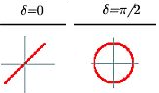
\includegraphics[scale=1]{fig1.png}
	\caption{Curvas que se obtendrán}
	\label{fig1}
\end{figure}

\section{Análisis y Resultados}
\noindent
Para esta práctica se implementarán tres circuitos los cuales  se muestran a continuación y sus cálculos correspondientes, además el diagrama fasorial. Para cada circuito se usara una fuente $AC$ con un $V_p=5\ V$  a una frecuencia $f = 1000\ Hz$.

\subsection{Circuito $RL$}
\noindent
Para el siguiente circuito se hace un análisis fasorial por el método de mallas
\begin{figure}[H]
	\centering
		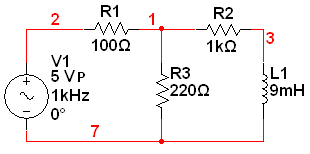
\includegraphics[scale=0.75]{circ1.png}
	\caption{Montaje del circuito $RL$}
	\label{fig2}
\end{figure}
\begin{equation}
 {Z_L} = j\omega L = j56.549
\label{ecu1}
\end{equation}
\begin{equation}
 5\angle 0^\circ  = {i_1}(100 + 220) - {i_2}(220)
\label{ecu2}
\end{equation}
\begin{equation}
 0 = {i_2}\left( {1000 + 220 + j56.549} \right) - {i_1}(220)
\label{ecu3}
\end{equation}
\noindent
Con la solución del sistema anterior se obtienen los siguientes datos:
\begin{table}[H]
	\centering
\begin{tabular}[c]{|c|c|c|} \hline
Elemento & Tensión $[V]$ & Corriente $[mA]$ \\ \hline
$R_1$ & $1.782 \angle -0.3748°$ & $17.83 \angle -0.3748°$ \\ \hline
$R_2$ & $3.2119 \angle -3.0288°$ & $3.2119 \angle -3.0288°$ \\ \hline
$R_3$ & $4.62836 \angle 0.14448°$ & $21.038 \angle 0.14448°$ \\ \hline
$L_1$ & $0.18163 \angle 86.971°$ & $3.2119 \angle -3.0288°$ \\ \hline
\end{tabular}
	\caption{Valores obtenidos teóricamente}
	\label{tab1}
\end{table}
\noindent
Luego se muestra el diagrama fasorial de la tensión y corriente en la inductancia, donde $V_L=Z_1$ y $I_L=Z_2$
\begin{figure}[H]
	\centering
		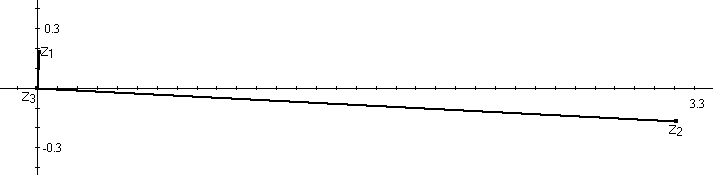
\includegraphics[scale=0.35]{fa1.png}
	\caption{Diagrama Fasorial circuito $RL$}
	\label{fig3}
\end{figure}
\noindent
Para desarrollar esta práctica con éxito se hizo necesario diseñar nuevamente los circuitos para obtener los resultados esperados.\\
Para el circuito $RL$ se utilizo el mismo circuito, pero se variaron los valores de las resistencias de la siguiente manera, $R_1 = 100\ \Omega$, $R_2 = 1\ K\Omega$, $R_3 = 2.185\ K\Omega$, resistencia de la bobina $R_L = 37.15\ \Omega$ a $9.0511\ mH$ en una frecuencia de $f=15.38\ KHz$.\\
\begin{figure}[H]
	\centering
		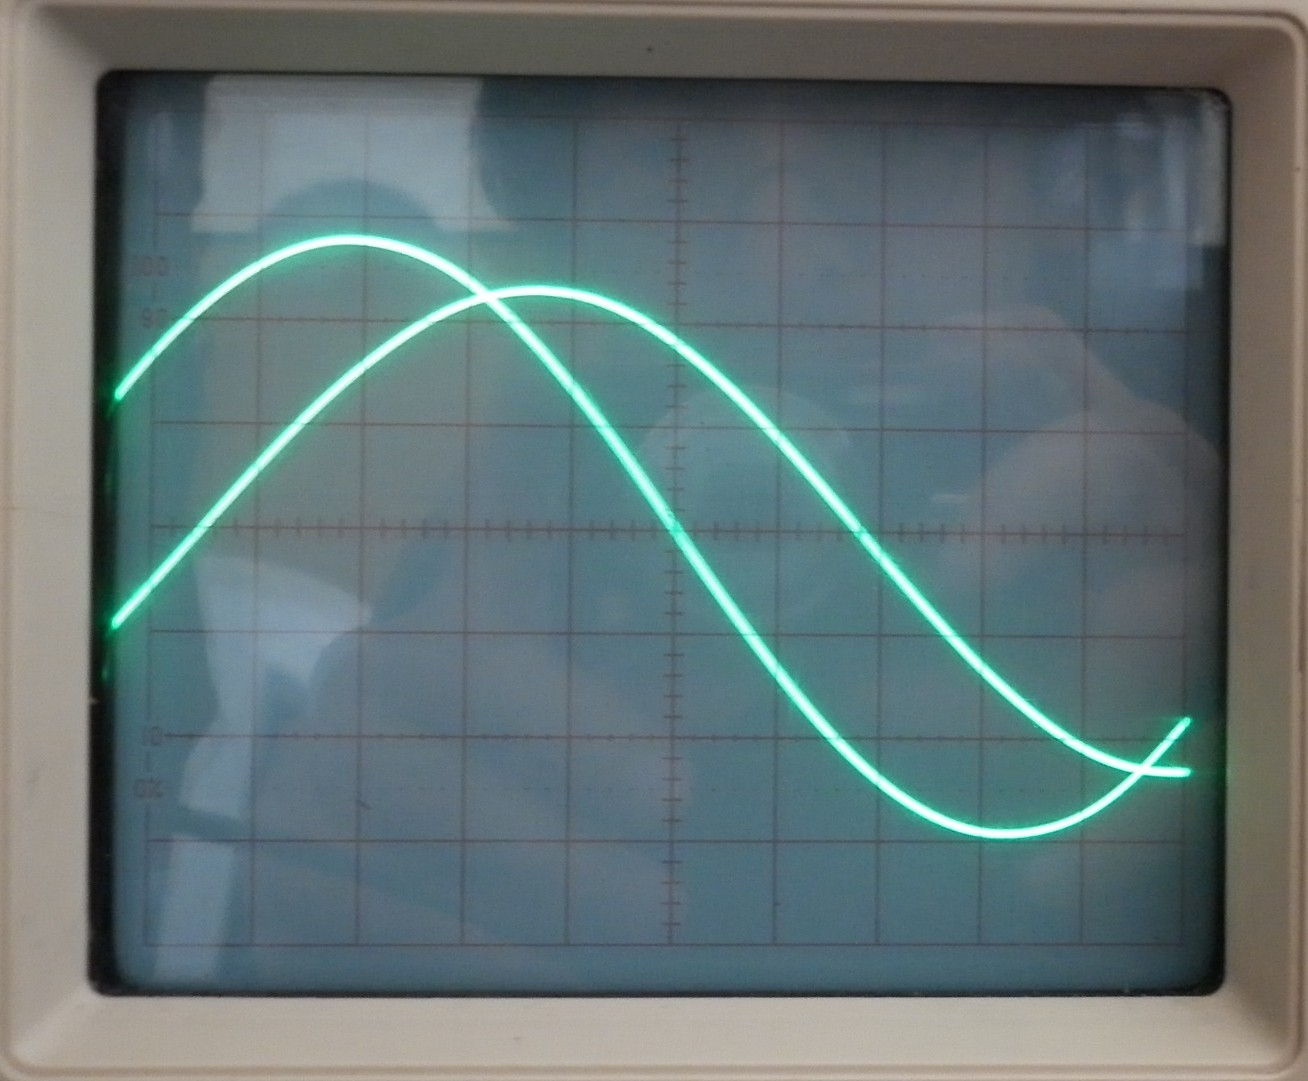
\includegraphics[scale=0.15]{232.png}
	\caption{Resultado del circuito RL}
	\label{figp1}
\end{figure}
\begin{figure}[H]
	\centering
		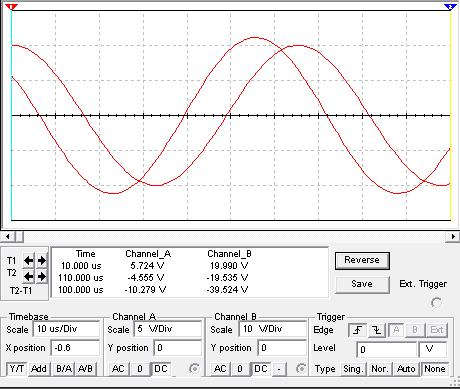
\includegraphics[scale=0.5]{RLsim.PNG}
	\caption{Simulación circuito RL}
	\label{fig1a}
\end{figure}
\noindent
Para las figuras de Lissajous los puntos de corte son $a = 9$, $b= 12$ y $t=8.5\ \mu s$.
\begin{figure}[H]
	\centering
		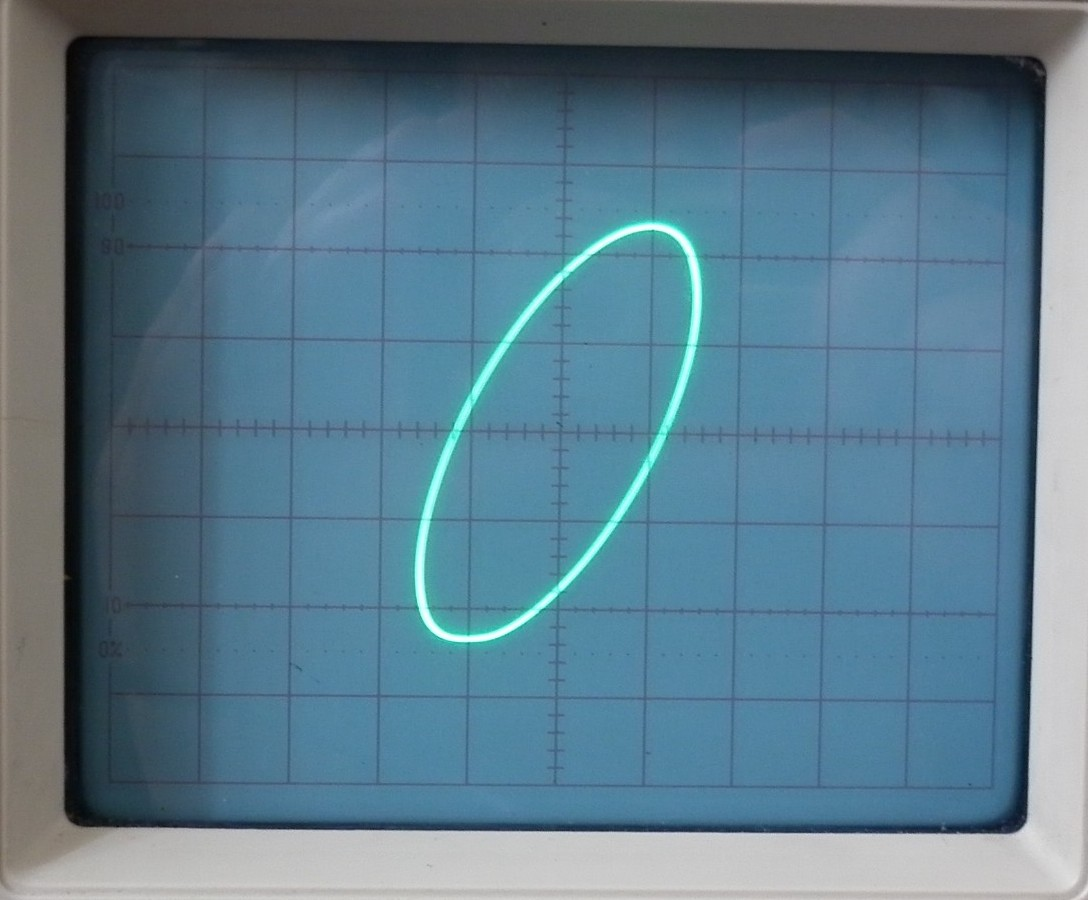
\includegraphics[scale=0.15]{233.png}
	\caption{Salida del circuito RL para la figura de Lissajous}
	\label{figp2}
\end{figure}
\noindent
Al analizar la Fig. \ref{fig1a} y observar el tiempo de desfase entre las dos señales medidas se puede observar un tiempo $t=10\ \mu s$\\ aproximadamente, este tiempo es cercano al obtenido experimentalmente el cual es de $t=8.5\ \mu s$.\\
Analizando la Fig. \ref{figp2} y basado en la ecu. (\ref{ecu100}) se obtiene un ángulo de desfase $\theta = 48.59 ^\circ$, luego analizando la Fig.\ref{figp1} y aplicando la ecu. (\ref{ecu101}) se obtuvo un ángulo de desfase de $\theta = 55.368 ^\circ$. Al comparar los ángulos obtenidos por los dos métodos, se puede decir que son aproximadamente iguales, a demás se tiene que la tensión se adelanta a la corriente.
\begin{equation}
 \theta = sin ^{-1} \frac{a}{b}
\label{ecu100}
\end{equation}
\begin{equation}
 \theta = t 2 \pi f
\label{ecu101}
\end{equation}

\subsection{CIRCUITO $RC$}
\noindent
Para este circuito se hace un análisis fasorial de por mallas.
\begin{figure}[H]
	\centering
		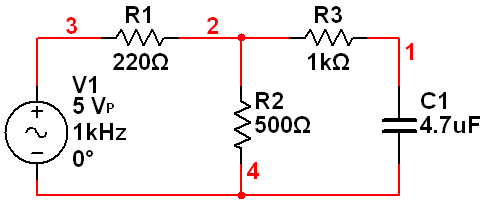
\includegraphics[scale=0.5]{circ2.png}
	\caption{Montaje del circuito $RL$}
	\label{fig4}
\end{figure}
\noindent
\begin{equation}
 Z_c = \frac{1}{{j\omega c}} =  - j33.863
\label{ecu4}
\end{equation}
\begin{equation}
 5\angle 0^\circ  = {i_1}(220 + 500) - {i_2}(500)
\label{ecu5}
\end{equation}
\begin{equation}
 0 = {i_2}\left( {1000 + 500 - j33.863} \right) - {i_1}(500)
\label{ecu6}
\end{equation}
\noindent
Al solucionar el sistema de ecuaciones se tiene los siguientes datos:
\begin{table}[H]
	\centering
\begin{tabular}[c]{|c|c|c|} \hline
Elemento & Tensión $[V]$ & Corriente $[mA]$ \\ \hline
$R_1$ & $1.987634 \angle -0.38929°$ & $9.0347 \angle -0.38929°$ \\ \hline
$R_2$ & $6.022 \angle -0.12854°$ & $12.044 \angle -0.12854°$ \\ \hline
$R_3$ & $3.30107 \angle 1.6826°$ & $3.30107 \angle 1.62826°$ \\ \hline
$C_1$ & $0.30594 \angle -89.611°$ & $9.0347 \angle 0.38929°$ \\ \hline
\end{tabular}
	\caption{Valores obtenidos teóricamente}
	\label{tab2}
\end{table}
\noindent
A continuación se tiene la gráfica fasorial de la corriente y la tensión en el capacitor, donde $V_C=Z_1$ y $I_C=Z_2$.
\begin{figure}[H]
	\centering
		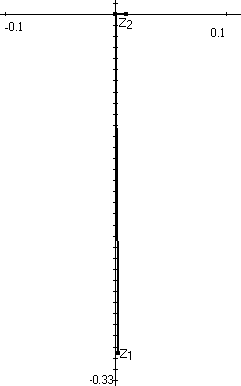
\includegraphics[scale=0.45]{fa2.png}
	\caption{Diagrama Fasorial circuito $RC$}
	\label{fig5}
\end{figure}
\noindent
Para el circuito $RC$ se utilizo el mismo circuito, pero se variaron los valores de las resistencias de la siguiente manera, $R_1 = 220\ \Omega$, $R_2 = 1.426\ K\Omega$, $R_3 = 1\ K\Omega$, resistencia en el condensador $R_C = 221.7\ \Omega$ a $49.313\ nF$ en una frecuencia de $f=1.126\ KHz$.\\
\begin{figure}[H]
	\centering
		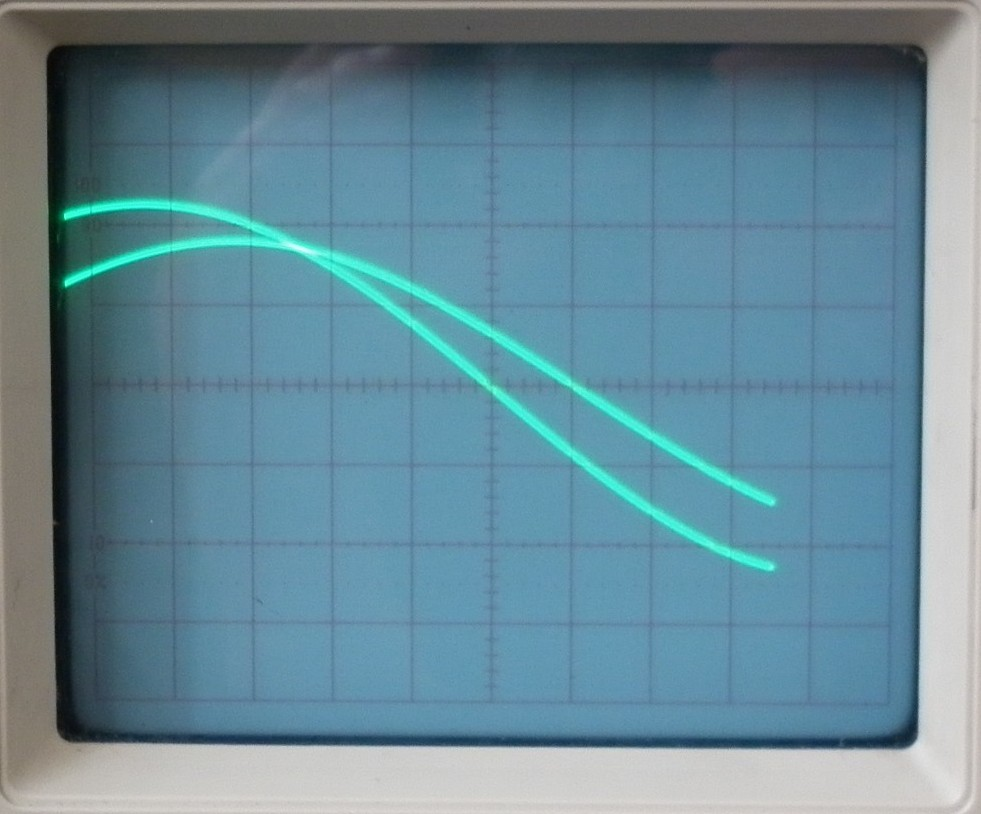
\includegraphics[scale=0.15]{234.png}
	\caption{Salida del circuito RC}
	\label{figp3}
\end{figure}
\begin{figure}[H]
	\centering
		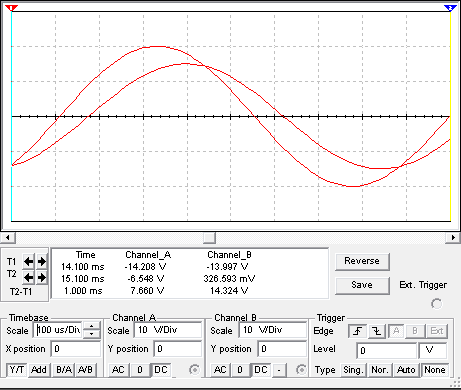
\includegraphics[scale=0.4]{RCsim.PNG}
	\caption{Simulación circuito RC}
	\label{fig1b}
\end{figure}
\noindent
Para las figuras de Lissajous los puntos de corte son $a = 4.5$, $b= 12$ y $t=50\ \mu s$
\begin{figure}[H]
	\centering
		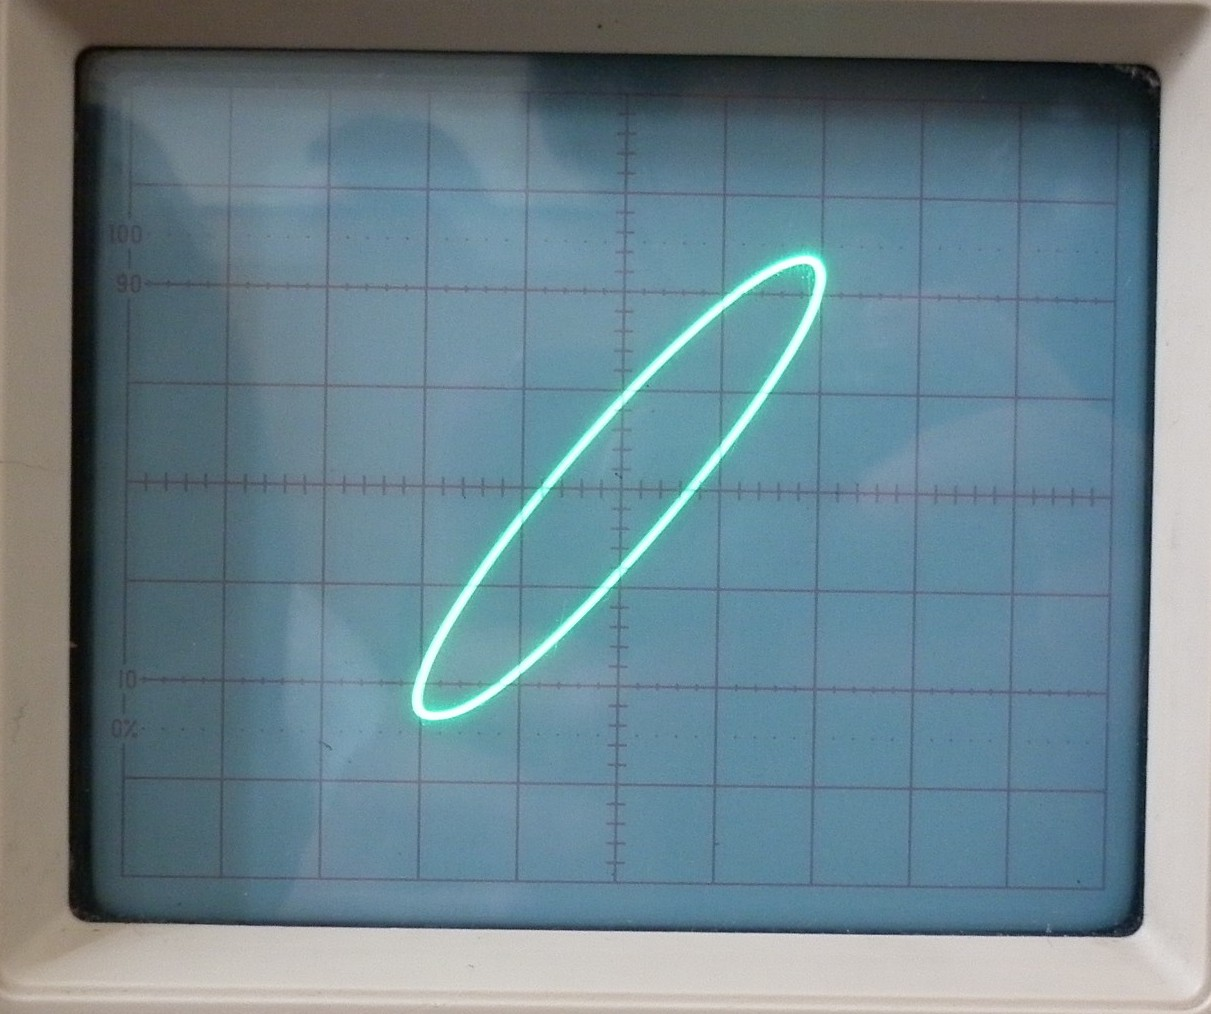
\includegraphics[scale=0.15]{235.png}
	\caption{Salida del circuito RC para la figura de Lissajous}
	\label{figp4}
\end{figure}
\noindent
Analizando las señales medidas en la Fig. \ref{fig1b} se puede observar un desfase aproximado en tiempo de $t=65\ \mu s$, el cual se acerca al valor obtenido experimentalmente que es de $t=50\ \mu s$.\\
Analizando la Fig. \ref{figp4} y basado en la ecu. (\ref{ecu100}) se obtiene un ángulo de desfase $\theta = 22.024 ^\circ$, luego analizando la Fig.\ref{figp3} y aplicando la ecu. (\ref{ecu101}) se obtuvo un ángulo de desfase de $\theta = 20.268 ^\circ$. Al comparar los ángulos obtenidos por los dos métodos, se puede decir que son aproximadamente iguales, a demás se tiene que la tensión se atrasa a la corriente.

\subsection{Circuito $RLC$}
\noindent
Para el siguiente circuito se hace un análisis fasorial por el método de mallas para observar el comportamiento del circuito en estado estacionario.
\begin{figure}[H]
	\centering
		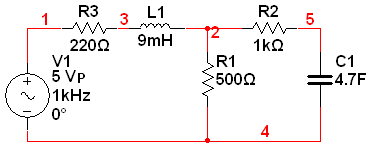
\includegraphics[scale=0.75]{circ3.png}
	\caption{Montaje del circuito $RLC$}
	\label{fig6}
\end{figure}
\begin{equation}
 Z_C = \frac{1}{{j\omega c}} =  - j33.863
\label{ecu7}
\end{equation}
\begin{equation}
 {Z_L} = j\omega L = j56.549
\label{ecu8}
\end{equation}
\begin{equation}
 5\angle 0^\circ  = {i_1}(220 + 500 + j56.549) - {i_2}(500)
\label{ecu9}
\end{equation}
\begin{equation}
 0=i_2 (1000+500-j33.863)-i_1 (500)
\label{ecu10}
\end{equation}
\noindent
A partir de la solución del sistema anterior se obtienen los siguientes datos:
\begin{table}[H]
	\centering
\begin{tabular}[c]{|c|c|c|} \hline
Elemento & Tensión $[V]$ & Corriente $[mA]$ \\ \hline
$R_1$ & $2.999 \angle -6.0938 ^\circ$ & $5.9979 \angle -6.0938^\circ$ \\ \hline
$R_2$ & $2.9972 \angle -4.1555^\circ$ & $2.9972 \angle -4.1555^\circ$ \\ \hline
$R_3$ & $1.9787 \angle -5.448^\circ$ & $8.994 \angle -5.448^\circ$ \\ \hline
$C_1$ & $0.10149 \angle -94.156^\circ$ & $0.0029978 \angle 4.1555^\circ$ \\ \hline
$C_1$ & $0.5089 \angle 84.552^\circ$ & $8.994 \angle -5.448^\circ$ \\ \hline
\end{tabular}
	\caption{Valores obtenidos teóricamente}
	\label{tab3}
\end{table}
\noindent
Para este circuito se tienen los diagramas fasoriales en $C_1$ y $L_1$.\\
Para este gráfico $V_C=Z_1$ y $I_C=Z_2$:
\begin{figure}[H]
	\centering
		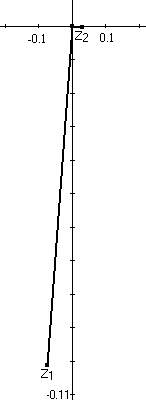
\includegraphics[scale=0.45]{fa3.png}
	\caption{Diagrama Fasorial circuito $RCL$}
	\label{fig7}
\end{figure}
\noindent
Para el siguiente diagrama se tiene que $V_L=Z_1$ y $I_L=Z_2$.
\begin{figure}[H]
	\centering
		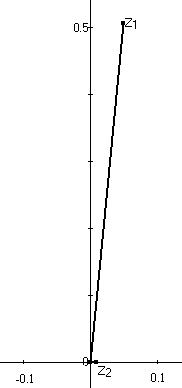
\includegraphics[scale=0.45]{fa4.png}
	\caption{Diagrama Fasorial circuito $RCL$}
	\label{fig8}
\end{figure}
\noindent
Para el circuito $RLC$ se utilizo el mismo circuito, pero se variaron los valores de las resistencias de la siguiente manera, $R_1 = 33.2\ \Omega$, $R_2 = 50\ \Omega$, $R_3 = 100|\ \Omega$, resistencia en el condensador $R_C = ???\ \Omega$ a $1000\ \mu F$, resistencia en el inductor $R_L = ???\ \Omega$ a $9\ mH$, en una frecuencia de $f=2\ MHz$.\\
\begin{figure}[H]
	\centering
		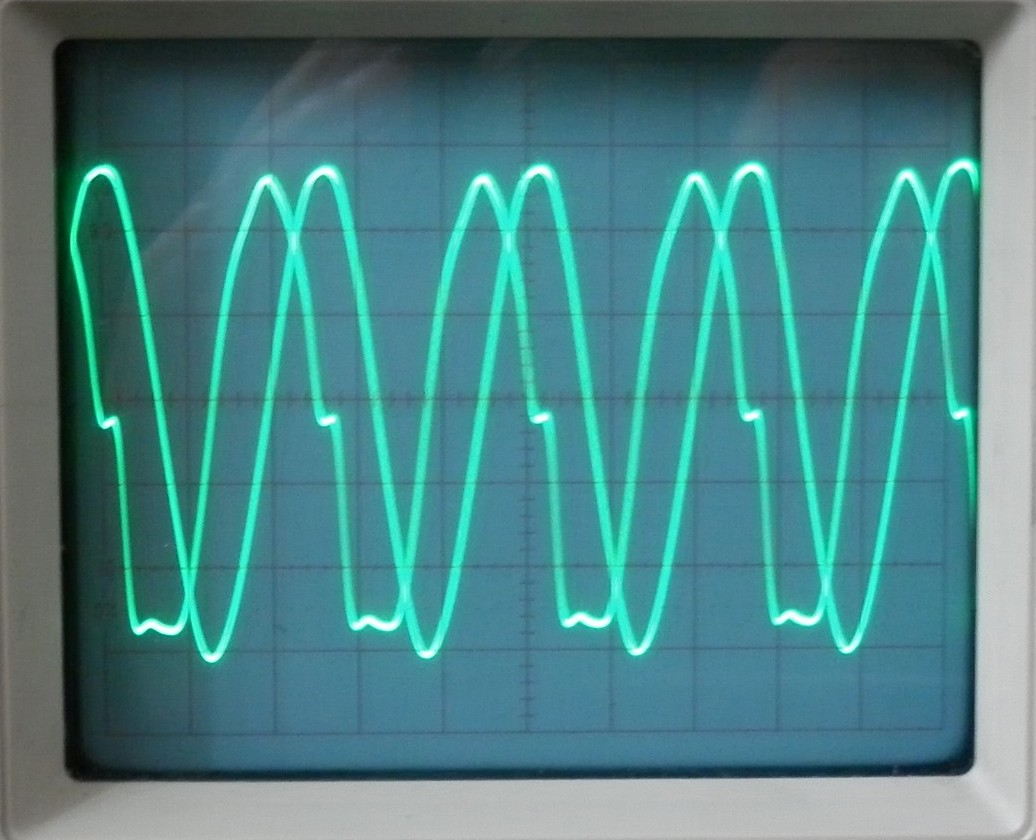
\includegraphics[scale=0.17]{236.png}
	\caption{Salida del circuito RLC}
	\label{figp5}
\end{figure}
\begin{figure}[H]
	\centering
		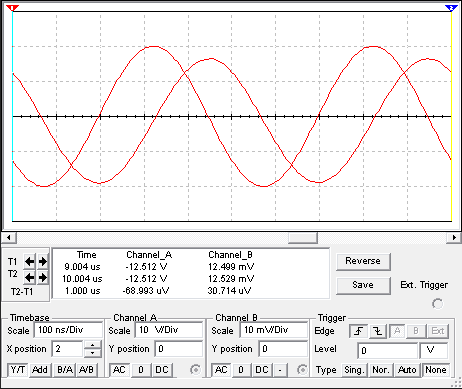
\includegraphics[scale=0.4]{RLCsim.PNG}
	\caption{Simulación circuito RLC}
	\label{fig1c}
\end{figure}
\noindent

Para las figuras de Lissajous los puntos de corte son $a = 6$, $b= 14$ y $t=0.14\ \mu s$.
\begin{figure}[H]
	\centering
		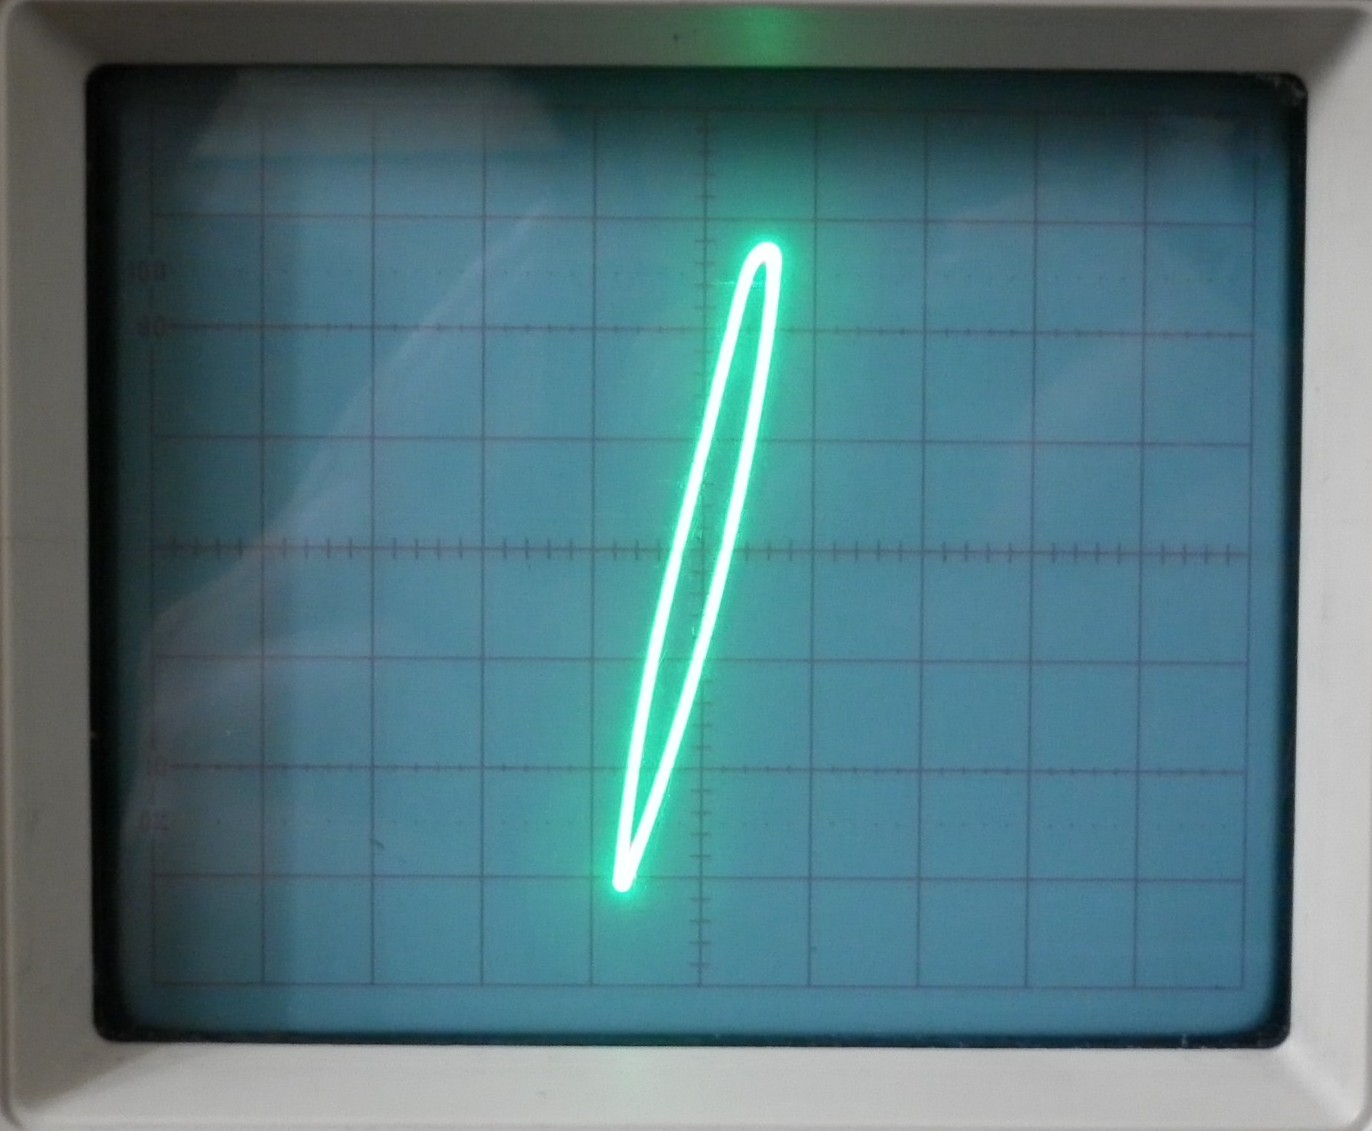
\includegraphics[scale=0.13]{237.png}
	\caption{Salida del circuito RLC para la figura de Lissajous}
	\label{figp6}
\end{figure}
\noindent
En la Fig. \ref{fig1c} se puede observar un desfase en tiempo entre las dos señales medidas de $t=0.13\ \mu s$, al comparar con el desfase obtenido en la práctica el cual es de $t=0.14\ \mu s$ se puede decir que son aproximadamente iguales.\\
Analizando la Fig. \ref{figp6} y basado en la ecu. (\ref{ecu100}) se obtiene un ángulo de desfase $\theta = 25.38 ^\circ$, luego analizando la Fig.\ref{figp5} y aplicando la ecu. (\ref{ecu101}) se obtuvo un ángulo de desfase de $\theta = 100.8 ^\circ$. Al comparar los ángulos obtenidos por los dos métodos, se puede decir que  no son iguales, posiblemente esto de debe a la frecuencia tan elevada que se utilizo.

\section{Preguntas}
\begin{enumerate}
 \item ¿Como es el ángulo de fase entre la tensión y la corriente de cada uno de los circuitos $RL$, $RC$ y $RLC$?\\
Elegimos una amplitud de tensión de la fuente de $V_M$ y un ángulo de fase de cero grados.\\
Para un circuito $RL$ el ángulo de fase de la corriente dependerá de la relación entre la tensión y la impedancia y como elegimos el ángulo de la fuente de tensión en cero grados, la corriente tendrá un ángulo de fase dependiente de la impedancia:
\begin{equation}
 \phi = -tan^{-1} \frac{\omega L}{R}
\label{ecu11}
\end{equation}
Utilizando la misma consideración para la fuente, en un circuito RC la corriente tendrá un ángulo de fase:
\begin{equation}
 \phi  =  - ta{n^{ - 1}}\frac{1}{{R\omega C}}
\label{ecu12}
\end{equation}
Para un circuito $RLC$ en serie tenemos que la corriente tendrá un ángulo de fase:
\begin{equation}
 \phi  =  - ta{n^{ - 1}}\frac{{\omega L - \frac{1}{{\omega C}}}}{R}
\label{ecu13}
\end{equation}

 \item ¿El ángulo de fase entre la tensión y la corriente en circuitos $RL$, $RC$ y $RLC$ varía con respecto a la frecuencia?\\
Si varía puesto que la impedancia del inductor y del condensador dependen directamente de la frecuencia:
\begin{equation}
 {Z_L} = j\omega L \ \ \ \ \ \ {Z_C} = \frac{1}{{j\omega C}}
\label{ecu14}
\end{equation}
\noindent
$\omega=2 \pi f$ siendo $f$ la frecuencia.

 \item ¿Que diferencias hay entre los ángulos medidos usando las figuras de Lissajous y usando la visualización en función del tiempo de osciloscopio?\\
Teóricamente deberían ser los mismos, pero por problemas de resolución del osciloscopio es más fácil revisar el ángulo cuando se visualizan las señales en función del tiempo, porque al utilizar el método de lissajous se hace difícil diferenciar los cortes con los ejes con mayor exactitud.
 \item ¿Que utilidad tiene el uso de los fasores en el análisis de circuitos en contraposición con los análisis realizados en las prácticas anteriores?\\
Las tensiones, corrientes e impedancias en un circuito de corriente alterna se pueden representar como vectores en el plano complejo, la notación fasorial toma los valores de magnitud y ángulo de dichos vectores y esto permite que los cálculos sean más cortos.
 \item ¿Coinciden las magnitudes y ángulos de fase obtenidos experimentalmente con los valores teóricos?\\
No coinciden con exactitud, pero se encuentran dentro de valores esperados. Esto es debido a que diferentes factores externos afectan al circuito, como la impedancia de la fuente o las capacitancias parasitas de los cables, además en el caso del condensador el aumento de la frecuencia representa un cambio en su comportamiento de elemento puro, ya que aparece un factor resistivo.
\end{enumerate}

\section{Conclusiones}
\begin{itemize}
 \item Cuando aumenta la frecuencia en el circuito $RC$, la tensión en el condensador disminuye esto se debe a la variación en su impedancia.
 \item Cuando aumenta la frecuencia en el circuito $RL$, la tensión en el inductor aumenta esto se debe a la variación en su impedancia.
 \item Nuestro modelo necesitaba frecuencias muy elevadas para funcionar y obtener los resultados esperados, a demás era muy difícil manipular una resistencia equivalente en paralelo, porque se presentaban problemas con las resistencias de las fuentes, multímetros y demás elementos, esto se vio reflejado al calcular el ángulo de desfase del circuito $RLC$, tanto para el método de Lissajous y para el método que depende del tiempo.
\end{itemize}

\bibliographystyle{ieeetran}
\begin{thebibliography}{99}
\bibitem{sadiku} Alexander, Charles K. \&  Sadiku, Matthew N.O.
{\em ```Fundamentals of Electric Circuits"'}.
McGRAW-HILL, ISE Editions, 1999.

\bibitem{dorf} Dorf  \& Svoboda.
{\em ```Circuitos Eléctricos"'}.
Alfaomega, Sexta Edición, 2006.

\bibitem{hayt} Hayt, William H. Jr., Kemmerly, Jack E. \& Durbin, Steven M.
{\em ```Análisis de circuitos en ingeniería"'}.
McGRAW-HILL, Séptima Edición, 2007.

\bibitem{nahvi} Nahvi, Mahmood \& Edminister, Joseph A.
{\em ```Theory and Problems of Electric Circuits"'}.
McGRAW-HILL, Fourth Edition, 2003.

\bibitem{page1} \url{http://es.wikipedia.org/wiki/Curva_de_Lissajous}. Visitada el 18 de septiembre de 2011.

\bibitem{page2} \url{http://www.chochitopelao.com/las-curvas-de-lissajous/}.
Visitada el 18 de septiembre de 2011.

\end{thebibliography}
\end{document} 